%=====================================================================
%  TriAnSec — IEEE Transactions Manuscript (Fully Corrected & Aligned)
%=====================================================================
\documentclass[journal,10pt]{IEEEtran}

% ---------- Core packages ----------
\usepackage{amsmath,amssymb,amsthm}
\usepackage{mathtools}
\usepackage{graphicx}
\usepackage{booktabs}
\usepackage{multirow}
\usepackage{array}
\usepackage{tabularx}
\usepackage{tikz}
\usetikzlibrary{positioning}
\usetikzlibrary{shapes.geometric,arrows.meta,positioning,fit,backgrounds,calc}
\usepackage{listings}
\usepackage{xcolor}
\usepackage{hyperref}
\usepackage{algorithm}
\usepackage{algpseudocode}
\usepackage{microtype}
\usepackage{balance}
\usepackage{url}
\usepackage{cite}
\usepackage{siunitx}
\setlength{\emergencystretch}{2em}

% ---------- Float tuning to keep figures close to their sections ----------
\usepackage{float}
\renewcommand{\topfraction}{0.95}
\renewcommand{\bottomfraction}{0.95}
\renewcommand{\textfraction}{0.05}
\renewcommand{\floatpagefraction}{0.85}
\renewcommand{\dbltopfraction}{0.95}
\renewcommand{\dblfloatpagefraction}{0.85}

% ---------- Hyperref ----------
\hypersetup{
    colorlinks=true,
    linkcolor=blue!60!black,
    citecolor=blue!60!black,
    urlcolor=blue!60!black,
    pdftitle={TriAnSec: A Stateful, Behavior-Driven Security Middleware for Application-Layer API Business Logic Protection},
    pdfauthor={Aniket Paswan, Anjali Jha, Anshika Pratap Singh}
}

% ---------- Theorem environments ----------
\newtheorem{definition}{Definition}
\newtheorem{theorem}{Theorem}
\newtheorem{lemma}{Lemma}
\newtheorem{proposition}{Proposition}
\newtheorem{remark}{Remark}

% ---------- Listings ----------
\definecolor{codebg}{RGB}{248,248,248}
\definecolor{codekw}{RGB}{0,0,180}
\definecolor{codestr}{RGB}{160,32,32}
\definecolor{codecmt}{RGB}{100,100,100}
\lstset{
    backgroundcolor=\color{codebg},
    basicstyle=\ttfamily\footnotesize,
    keywordstyle=\color{codekw}\bfseries,
    stringstyle=\color{codestr},
    commentstyle=\color{codecmt}\itshape,
    numbers=left,
    numberstyle=\tiny\color{codecmt},
    frame=single,
    breaklines=true,
    captionpos=b,
    tabsize=2
}

% ---------- Convenience macros ----------
\newcommand{\Fclient}{\mathcal{F}_{\mathrm{client}}}
\newcommand{\Ktenant}{K_{\mathrm{tenant}}}
\newcommand{\Ucookie}{U_{\mathrm{cookie}}}
\newcommand{\Tfast}{\tau_{\mathrm{fast}}}
\newcommand{\ip}{IP_{\mathrm{src}}}
\newcommand{\ewma}{\mathrm{EWMA}}
\newcommand{\trust}{T_t}
\newcommand{\burst}{B_t}
\newcommand{\patt}{P_t}
\newcommand{\hist}{H_t}
\newcommand{\viol}{V_t}

%=====================================================================
\begin{document}

\title{TriAnSec: A Stateful, Behavior-Driven Security Middleware for\\
Application-Layer API Business Logic Protection}

\author{
\IEEEauthorblockN{Aniket Paswan, Anjali Jha, and Anshika Pratap Singh}
\IEEEauthorblockA{Department of Computer Science and Engineering\\
Galgotias College of Engineering and Technology (GCET),\\
Greater Noida, Uttar Pradesh, India\\
Affiliated with Dr.\ A.P.J.\ Abdul Kalam Technical University (AKTU), Lucknow, India\\
Supervised by: Ms.\ Ramandeep Kaur and Dr.\ Amrita Jyoti (HOD CSE)}
}

\maketitle

%=====================================================================
\begin{abstract}
While infrastructure-level edge defenses---Content Delivery Networks (CDNs), L3/L4 volumetric DDoS scrubbers, and Cloudflare-style edge firewalls---successfully mitigate network floods and coarse syntax anomalies, they remain fundamentally blind to \emph{application-layer business logic abuse}. Sophisticated automated botnets, credential stuffers, and scrapers routinely bypass edge filters by operating below static rate thresholds, distributing requests across residential proxy networks, and emitting syntactically valid HTTP transactions that mimic human interaction. Once past the perimeter, these campaigns target high-value workflows (authentication, checkout, OTP generation, and proprietary data endpoints). Existing in-application protections rely on single-counter rate limiters (Fixed-Window, Sliding-Log) that evaluate clients solely by source IP address ($\ip$); this yields catastrophic False-Positive Rates (FPR) for legitimate users behind Carrier-Grade NAT (CGNAT) gateways while providing \textbf{0.00\% detection recall} against distributed, low-and-slow adversaries.

We present \textbf{TriAnSec}, a stateful, behavior-driven API security platform designed to operate \emph{behind} edge infrastructure as an in-process application middleware. TriAnSec decouples real-time enforcement from compute-intensive behavioral analysis through a \textbf{Dual-Path Execution Model}: an ultra-low-latency synchronous fast path governed by an atomic Redis Lua script, coupled with an asynchronous, non-blocking \emph{fire-and-forget} intelligence pipeline. Clients are no longer isolated IP counters but persistent digital identities constructed from an entropy-weighted multi-signal model combining W3C HTTP Client Hints (\texttt{Sec-CH-UA-*}), cryptographically signed session cookies, and request-pattern vectors. Historical suspicion is smoothed via Exponentially Weighted Moving Averages (EWMA) and dynamic tenant-isolated adaptive thresholds, powering a progressive tri-state enforcement policy ($\mathrm{ALLOW}\!\to\!\mathrm{THROTTLE}\!\to\!\mathrm{BLOCK}$) with structured RFC~7231 explainability.

Across multi-run empirical trials against an industry-standard Fixed-Window application limiter and three systematic architectural ablations, TriAnSec achieves an \textbf{F1-score of $0.966\pm0.009$}, \textbf{$95.03\%\pm0.46\%$ recall on malicious traffic}, \textbf{$98.31\%\pm1.44\%$ precision}, \textbf{$3.00\%\pm2.37\%$ FPR}, and a median fast-path decision latency of $\mathbf{4.26\pm0.45\ \text{ms}}$. Under identical conditions, the Fixed-Window baseline collapses to \textbf{0.00\% recall} across $2{,}615$ adversarial IP shifts. Removing Client Hints from the identity resolver causes FPR to surge more than fivefold to \textbf{16.16\%}, proving that multi-signal behavioral intelligence is essential for modern business-logic defense.
\end{abstract}

\begin{IEEEkeywords}
API security, business logic abuse, behavior-driven security, EWMA trust scoring, application-layer rate limiting, Redis Lua, W3C Client Hints, dual-path architecture, ASGI middleware, OWASP API4/API6.
\end{IEEEkeywords}

%=====================================================================
\section{Introduction}
\IEEEPARstart{M}{odern} digital platforms, SaaS ecosystems, and microservice architectures are fundamentally glued together by Application Programming Interfaces (APIs)~\cite{nist2020}. As APIs have become the central operational backbone of enterprise software, their open nature has transformed them into the primary attack surface for automated cyber threats. Securing critical backend business logic without degrading system performance or disrupting legitimate users is now a first-order engineering challenge.

Automated campaigns---credential stuffing (OWASP API2), inventory scraping, automated account creation, and business workflow exploitation (OWASP API6)~\cite{owasp2023}---increasingly emulate legitimate human traffic patterns. A layered \emph{Defense-in-Depth} posture (Fig.~\ref{fig:layered}) is therefore required: Layer~1 (Edge) absorbs volumetric attacks, while Layer~2 (Application) must distinguish authentic interaction from abuse within a running business process.

\begin{figure}[!t]
\centering
\resizebox{\columnwidth}{!}{%
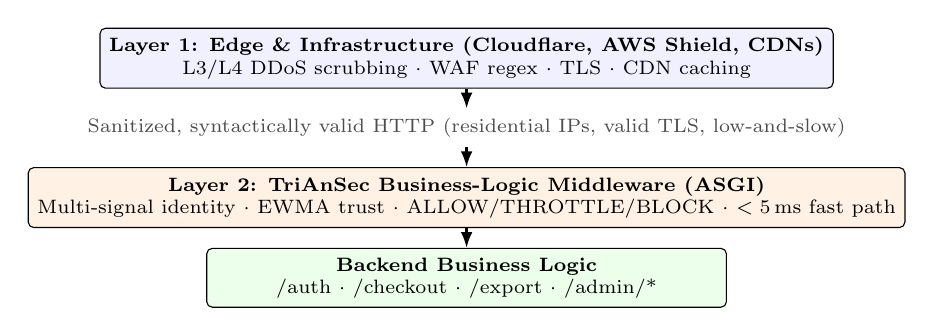
\begin{tikzpicture}[
    box/.style={draw, rounded corners=2pt, align=center, font=\scriptsize, minimum width=6.6cm, minimum height=0.55cm, fill=white},
    l1/.style={box, fill=blue!6},
    l2/.style={box, fill=orange!10},
    l3/.style={box, fill=green!8},
    arr/.style={-{Latex[length=2mm]}, thick}
]
\node[l1] (edge) {\textbf{Layer 1: Edge \& Infrastructure (Cloudflare, AWS Shield, CDNs)}\\ L3/L4 DDoS scrubbing $\cdot$ WAF regex $\cdot$ TLS $\cdot$ CDN caching};
\node[below=0.25cm of edge, font=\scriptsize, align=center, text=black!70] (mid) {Sanitized, syntactically valid HTTP (residential IPs, valid TLS, low-and-slow)};
\node[l2, below=0.25cm of mid] (tri) {\textbf{Layer 2: TriAnSec Business-Logic Middleware (ASGI)}\\ Multi-signal identity $\cdot$ EWMA trust $\cdot$ ALLOW/THROTTLE/BLOCK $\cdot$ $<5$\,ms fast path};
\node[l3, below=0.25cm of tri] (app) {\textbf{Backend Business Logic}\\ /auth $\cdot$ /checkout $\cdot$ /export $\cdot$ /admin/*};
\draw[arr] (edge) -- (mid);
\draw[arr] (mid) -- (tri);
\draw[arr] (tri) -- (app);
\end{tikzpicture}%
}
\caption{Defense-in-depth architecture. TriAnSec operates \emph{behind} edge infrastructure to protect application workflows that appear syntactically valid to edge firewalls.}
\label{fig:layered}
\end{figure}

\subsection{Why Edge Defenses Cannot Protect Business Logic}
Edge platforms excel at perimeter availability: absorbing multi-gigabit L3/L4 floods, terminating TLS, caching static assets, and applying broad regex WAF signatures. They are structurally blind to business-logic abuse because:
\begin{itemize}
    \item \textbf{Valid semantics.} Credential stuffing and scraping use standard HTTP verbs with valid parameters; no signature rule is violated.
    \item \textbf{Residential proxy infiltration.} Requests originate from clean residential ISP IPs (e.g., BrightData, Oxylabs)~\cite{mi2019resident}, defeating IP reputation lists.
    \item \textbf{Contextual blindness.} Edge CDNs have no visibility into tenant-level API permissions, database execution cost, session cookie state, or user behavioral trajectories.
\end{itemize}

\subsection{Mathematical Deficits of Conventional Rate Limiters}
Existing in-application rate limiters (e.g., \texttt{slowapi}, \texttt{express-rate-limit}, static Redis counters) evaluate a request $R_t$ arriving at time $t$ from source IP $I$:
\begin{equation}
\sum_{\tau=t-W}^{t} C_I(\tau) \;\le\; N_{\mathrm{threshold}},
\label{eq:baseline}
\end{equation}
where $W$ is the window and $N_{\mathrm{threshold}}$ is a static cap. This formulation fails catastrophically in two regimes:

\textbf{(i) CGNAT false positives.} With $K$ legitimate users sharing a public IP via Carrier-Grade NAT,
\begin{equation}
\sum_{k=1}^{K}\lambda_k > N_{\mathrm{threshold}}
\;\Longrightarrow\;
\text{blanket lockout of all users.}
\end{equation}

\textbf{(ii) Distributed evasion.} An adversary across $M$ residential proxy nodes such that each node satisfies
\begin{equation}
\sum_{\tau=t-W}^{t}C_{I_i}(\tau) < N_{\mathrm{threshold}} \quad \forall i\in[1,M]
\end{equation}
still produces aggregate rate
\begin{equation}
\sum_{i=1}^{M}\!\Big(\!\sum_{\tau=t-W}^{t}C_{I_i}(\tau)\!\Big) \gg N_{\mathrm{threshold}},
\end{equation}
yielding \textbf{0.00\% detection recall}.

\subsection{The TriAnSec Shift}
TriAnSec abandons the counter question \emph{``has this IP exceeded $N$?''} and poses the behavioral question \emph{``given the client's multi-signal identity, entropy, historical trust, and tenant context, should this request reach business logic?''} Table~\ref{tab:comparison} summarizes the architectural contrast.

\begin{table*}[!t]
\centering
\caption{Architectural Positioning: Traditional Limiters vs.\ Edge WAFs vs.\ TriAnSec}
\label{tab:comparison}
\renewcommand{\arraystretch}{1.18}
\begin{tabularx}{\textwidth}{@{}lXXX@{}}
\toprule
\textbf{Dimension} & \textbf{Traditional App Limiter} & \textbf{Edge WAF / CDN} & \textbf{TriAnSec (Ours)} \\
\midrule
Operational layer     & L7 app middleware              & L3/4/7 edge perimeter         & \textbf{L7 business-logic middleware} \\
Primary scope         & Numerical counting             & Volumetric + caching          & \textbf{Workflow abuse mitigation} \\
Identity model        & Single source IP               & IP + TLS fingerprint          & \textbf{Hints + cookies + fingerprint} \\
Enforcement           & Binary (drop/allow)            & Block / CAPTCHA               & \textbf{Progressive ALLOW$\to$THROTTLE$\to$BLOCK} \\
Decision latency      & $<2$\,ms                       & Edge ($0$\,ms backend)        & \textbf{P50 $=4.26$\,ms} \\
IP-rotation recall    & \textbf{0.00\%}                & Ineffective (residential)     & \textbf{95.03\% (2,337 shifts)} \\
Explainability        & Opaque 429                     & Generic error page            & \textbf{RFC 7231 + JSON reasons} \\
\bottomrule
\end{tabularx}
\end{table*}

\subsection{Contributions}
Our contributions are:
\begin{enumerate}
    \item \textbf{Architecture.} A dual-path execution model reconciling sub-5ms synchronous enforcement with compute-intensive asynchronous behavioral intelligence via an atomic single-RTT Redis Lua script and non-blocking fire-and-forget background pipeline.
    \item \textbf{Identity.} An entropy-weighted multi-signal identity tuple ($\Ktenant$, $\Ucookie$, $\Fclient$, $\ip$) that defeats IP rotation without client-side JavaScript.
    \item \textbf{Formalization.} A closed-form trust formulation combining burst velocity, pattern anomaly, EWMA historical suspicion, and normalized violations, with tenant-adaptive dynamic thresholds and a tri-state progressive policy.
    \item \textbf{Rigor.} A reproducible multi-run benchmark harness (63 concurrent clients, 500+ public IP pool, per-request telemetry of 22 attributes) with $i.i.d.$ cold-start guarantees, and three architectural ablations isolating signal contributions.
    \item \textbf{Empirical evidence.} F1 $=0.966\pm0.009$, recall $=95.03\%\pm0.46\%$, FPR $=3.00\%\pm2.37\%$, and P50 latency $=4.26\pm0.45$\,ms, establishing the first-order necessity of multi-signal behavioral defense.
\end{enumerate}

%=====================================================================
% CRITICAL LATEX PLACEMENT FIX:
% In IEEEtran, two-column floats (\begin{figure*}) CANNOT be output on the
% same page where they are declared. Defining Figure 2 (Full Architecture)
% here at the end of Section I forces LaTeX to queue it and typeset it at the
% top of Page 2, exactly where Section III / IV is introduced!
%=====================================================================
\begin{figure*}[!t]
\centering
\resizebox{0.92\textwidth}{!}{%
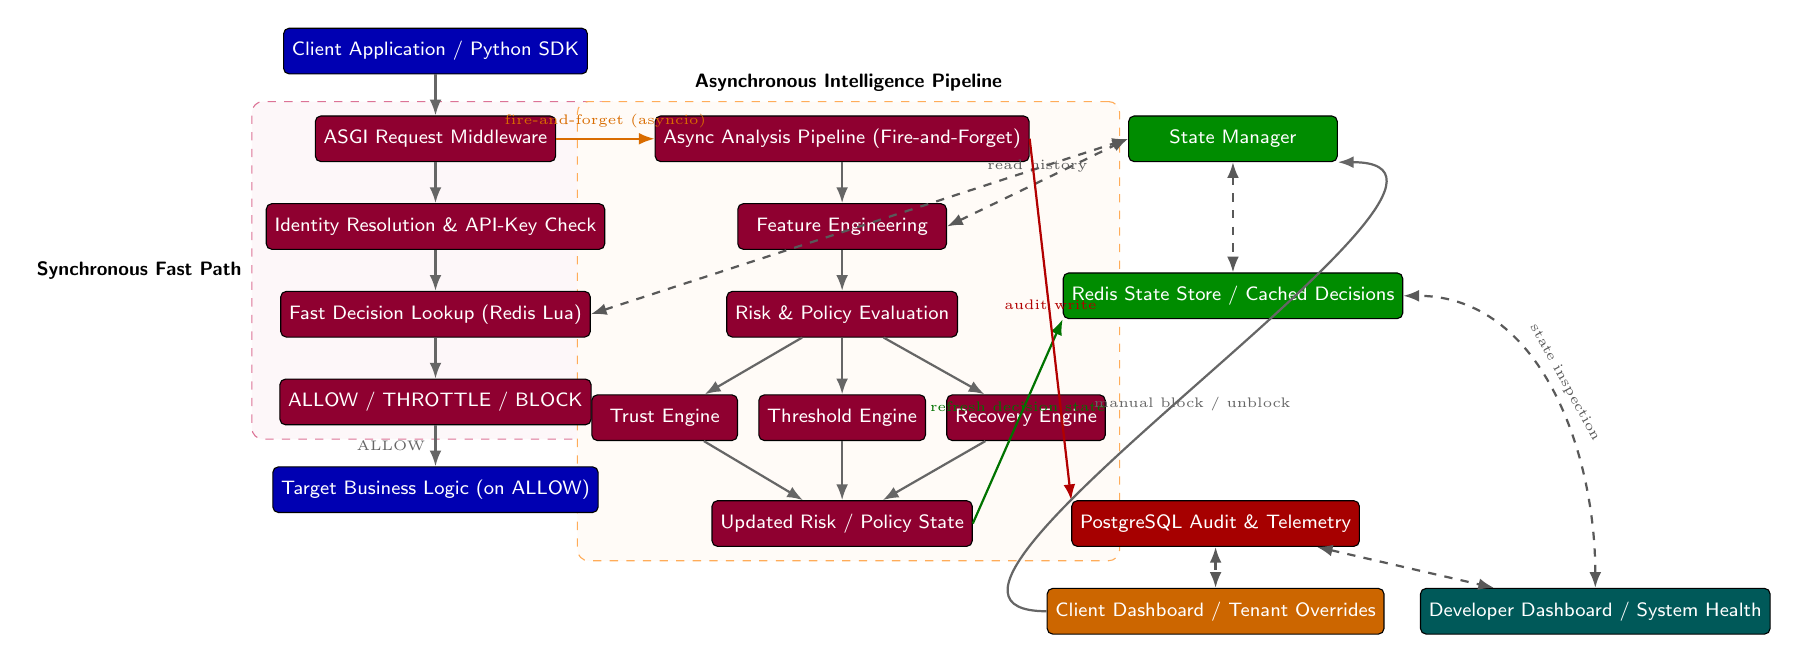
\begin{tikzpicture}[
    node distance=0.52cm and 1.25cm,
    block/.style={draw, rounded corners=2pt, align=center, minimum height=0.58cm, minimum width=2.65cm, text=white, font=\sffamily\scriptsize, inner sep=3pt},
    smallblock/.style={draw, rounded corners=2pt, align=center, minimum height=0.58cm, minimum width=1.85cm, text=white, font=\sffamily\scriptsize, inner sep=3pt},
    flow/.style={-{Latex[length=2mm]}, thick, gray!80!black},
    stateflow/.style={{Latex[length=2mm]}-{Latex[length=2mm]}, thick, dashed, gray!70!black}
]
% Synchronous request path
\node[block, fill=blue!70!black] (client) {Client Application / Python SDK};
\node[block, fill=purple!75!black, below=of client] (mw) {ASGI Request Middleware};
\node[block, fill=purple!75!black, below=of mw] (identity) {Identity Resolution \& API-Key Check};
\node[block, fill=purple!75!black, below=of identity] (gate) {Fast Decision Lookup (Redis Lua)};
\node[block, fill=purple!75!black, below=of gate] (enforce) {ALLOW / THROTTLE / BLOCK};
\node[block, fill=blue!70!black, below=of enforce] (app) {Target Business Logic (on ALLOW)};

% Asynchronous analysis pipeline
\node[block, fill=purple!75!black, right=of mw] (worker) {Async Analysis Pipeline (Fire-and-Forget)};
\node[block, fill=purple!75!black, below=of worker] (features) {Feature Engineering};
\node[block, fill=purple!75!black, below=of features] (policy) {Risk \& Policy Evaluation};
\node[smallblock, fill=purple!75!black, below left=0.72cm and -0.15cm of policy] (trust) {Trust Engine};
\node[smallblock, fill=purple!75!black, below=0.72cm of policy] (threshold) {Threshold Engine};
\node[smallblock, fill=purple!75!black, below right=0.72cm and -0.15cm of policy] (recovery) {Recovery Engine};
\node[block, fill=purple!75!black, below=0.75cm of threshold] (updated) {Updated Risk / Policy State};

% State and persistence
\node[block, fill=green!55!black, right=of worker] (manager) {State Manager};
\node[block, fill=green!55!black, below=1.4cm of manager] (redis) {Redis State Store / Cached Decisions};
\node[block, fill=red!65!black, right=of updated] (db) {PostgreSQL Audit \& Telemetry};
\node[block, fill=orange!80!black, below=of db] (clientdash) {Client Dashboard / Tenant Overrides};
\node[block, fill=teal!70!black, right=0.45cm of clientdash] (devdash) {Developer Dashboard / System Health};

% Grouping boxes
\begin{scope}[on background layer]
  \node[draw=purple!55, fill=purple!3, dashed, rounded corners, fit=(mw) (identity) (gate) (enforce), inner sep=5pt,
    label={[font=\sffamily\scriptsize\bfseries]left:Synchronous Fast Path}] {};
  \node[draw=orange!65, fill=orange!3, dashed, rounded corners, fit=(worker) (features) (policy) (trust) (threshold) (recovery) (updated), inner sep=5pt,
    label={[font=\sffamily\scriptsize\bfseries]above:Asynchronous Intelligence Pipeline}] {};
\end{scope}

% Main request flow
\draw[flow] (client) -- (mw);
\draw[flow] (mw) -- (identity);
\draw[flow] (identity) -- (gate);
\draw[flow] (gate) -- (enforce);
\draw[flow] (enforce) -- node[left, font=\tiny, align=right] {ALLOW} (app);

% Decision state read and asynchronous processing
\draw[stateflow] (gate.east) -- (manager.west);
\draw[stateflow] (manager) -- (redis);
\draw[flow, orange!85!black] (mw.east) -- node[above, font=\tiny] {fire-and-forget (asyncio)} (worker.west);
\draw[flow] (worker) -- (features);
\draw[flow] (features) -- (policy);
\draw[flow] (policy) -- (trust);
\draw[flow] (policy) -- (threshold);
\draw[flow] (policy) -- (recovery);
\draw[flow] (trust) -- (updated);
\draw[flow] (threshold) -- (updated);
\draw[flow] (recovery) -- (updated);
\draw[stateflow] (features.east) -- node[above, font=\tiny] {read history} (manager.west);
\draw[flow, green!45!black] (updated.east) -- node[above, font=\tiny] {refresh decision state} (redis.south west);
\draw[flow, red!70!black] (worker.east) -- node[above, font=\tiny] {audit write} (db.north west);
\draw[stateflow] (db) -- (clientdash);
\draw[stateflow] (db) -- (devdash);
\draw[flow] (clientdash.west) to[out=180,in=0] node[below, font=\tiny] {manual block / unblock} (manager.south east);
\draw[stateflow] (devdash.north) to[out=90,in=0] node[above, sloped, font=\tiny] {state inspection} (redis.east);
\end{tikzpicture}%
}
\caption{TriAnSec end-to-end architecture showing the synchronous fast path ($\Tfast < 5$\,ms), non-blocking asynchronous behavioral intelligence, atomic Redis decision updates, and dual operational dashboards.}
\label{fig:full-architecture}
\end{figure*}

%=====================================================================
\section{Related Work \& Theoretical Foundations}
\label{sec:related}

\paragraph{OWASP API taxonomy.} The OWASP API Top~10 designates \emph{Unrestricted Resource Consumption} (API4) and \emph{Unrestricted Access to Sensitive Business Flows} (API6)~\cite{owasp2023} as critical vulnerabilities. Attackers exploit business logic by remaining below volumetric thresholds; TriAnSec monitors behavioral access entropy on specific business endpoints.

\paragraph{Stateless transport limits.} Fielding and Reschke established that HTTP/1.1 is intrinsically stateless~\cite{rfc7231}; native web servers cannot maintain session risk trajectories without external state stores. We build on RFC~7231 and RFC~6585~\cite{rfc6585} to introduce explainable telemetry headers and RFC-compliant throttling responses.

\paragraph{In-memory state engines.} In-memory data structures (Redis sorted sets, state hashes) provide sub-millisecond latency~\cite{redis2024}, making Redis the natural real-time state repository for fast-path gating.

\paragraph{Proxy evasion.} Ramirez~\cite{ramirez2022} and Mi et al.~\cite{mi2019resident} demonstrate that botnets routinely bypass token-bucket limiters by distributing requests across residential IP proxy networks, rendering single-signal IP tracking structurally obsolete.

\paragraph{Behavioral anomaly detection.} Reis et al.~\cite{reis2022} show that multi-attribute behavioral analysis materially reduces false positives versus static thresholds. TriAnSec extends this line by formalizing an EWMA trust-decay engine paired with dynamic tenant thresholding, and by empirically ablating each signal.

%=====================================================================
\section{Threat Model \& Design Goals}
\label{sec:threat}

\subsection{Adversary Capabilities}
We assume a rational, adaptive adversary capable of:
\begin{itemize}
    \item \textbf{(A1) Source-IP rotation} across $\mathcal{O}(10^3)$ residential and mobile IPs at arbitrary cadence.
    \item \textbf{(A2) HTTP-layer mimicry} of legitimate clients (headers, verbs, request bodies, User-Agent variety).
    \item \textbf{(A3) Cookie churn}, i.e., discarding persistent session state between requests.
    \item \textbf{(A4) Client Hint spoofing} via customized browser builds or headless Chromium.
    \item \textbf{(A5) Low-and-slow volleys}: burst patterns below static per-IP thresholds.
\end{itemize}

\subsection{Out-of-Scope Adversaries}
TriAnSec does \emph{not} claim to defend against: volumetric L3/L4 DDoS (edge's mandate), TLS-layer attacks, application code-level exploits (SQLi/XSS/RCE), or fully coordinated multi-account adversaries who emulate human timing distributions with clean Client Hints. These are discussed in Sec.~\ref{sec:limits}.

\subsection{Security Goals}
\begin{description}
    \item[G1] \textbf{Recall $\ge 90\%$} on distributed malicious traffic while \textbf{FPR $\le 5\%$} on legitimate CGNAT-bound users.
    \item[G2] \textbf{P50 fast-path latency $\le 5$\,ms} at ${>}40$\,req/s sustained throughput.
    \item[G3] \textbf{Progressive enforcement}: adversaries blocked, borderline actors throttled, not carpet-bombed.
    \item[G4] \textbf{Explainability} per RFC~7231: every interception emits a structured reason and \texttt{Retry-After}.
    \item[G5] \textbf{Tenant isolation}: no cross-tenant state leakage in shared Redis clusters.
\end{description}

%=====================================================================
\section{System Architecture \& Dual-Path Design}
\label{sec:arch}

TriAnSec is architected as an ASGI middleware component that integrates seamlessly into modern asynchronous Python web frameworks (FastAPI, Starlette, Quart, Django Channels). Listing~\ref{lst:sdk-integration} illustrates the zero-boilerplate developer integration pattern.

\begin{lstlisting}[language=Python, caption={Minimal TriAnSec ASGI middleware integration interface.}, label={lst:sdk-integration}, basicstyle=\ttfamily\scriptsize]
from fastapi import FastAPI
from triansec import SecurityMiddleware

app = FastAPI(title="Production Microservice API")

# Single-statement ASGI middleware attachment
app.add_middleware(
    SecurityMiddleware,
    tenant_id="tenant_prod_corp_01",
    api_key="ts_live_demo_xxxxxxxxxxxxxxxxxxxxxx",
    fail_open=True,  # Gracefully ALLOW if state store fails
)
\end{lstlisting}

\subsection{Dual-Path Execution Model}
To reconcile deep behavioral analytics with strict microservice SLAs, the execution plane is decoupled into two paths (Fig.~\ref{fig:seq-single-col}):

\paragraph{Synchronous fast path ($\mathcal{O}(1)$).}
Intercepts each request at the ASGI boundary. It: (i) resolves tenant identity via an in-memory SHA-256 API-key cache, avoiding database I/O; (ii) dispatches an atomic Redis \texttt{EVALSHA} against the pre-computed identity state hash $\{base\}{:}state$; and (iii) returns the pre-rendered verdict \emph{immediately} before \texttt{await call\_next(request)}. Latency is strictly measured from socket arrival to verdict delivery:
\begin{equation}
\Tfast \;=\; t_{\mathrm{decision\_served}} \;-\; t_{\mathrm{request\_arrival}}.
\label{eq:tau}
\end{equation}

\paragraph{Asynchronous fire-and-forget intelligence pipeline.}
Rather than blocking the client response, background behavioral analysis is dispatched as an asynchronous \emph{fire-and-forget} coroutine using \texttt{asyncio.ensure\_future()}. The ASGI response is flushed immediately to the network socket. To prevent algorithmic amplification and queue saturation under distributed floods:
\begin{enumerate}
    \item \textbf{Rejection-path deduplication:} An in-memory cache (\texttt{\_should\_spawn\_rejection\_task}) limits background audit executions for blocked identities to at most one per 30-second window.
    \item \textbf{Non-blocking error trapping:} A bound completion callback logs any unexpected coroutine exceptions without generating orphaned unhandled task warnings.
    \item \textbf{State refresh:} The coroutine extracts request features, evaluates the risk and trust engines, and updates the Redis state hash $\{base\}{:}state$ so that subsequent requests immediately read the refreshed verdict on the fast path.
\end{enumerate}

% SINGLE COLUMN SEQUENCE DIAGRAM (Fixes layout and float page-jumping)
\begin{figure}[!t]
\centering
\resizebox{\columnwidth}{!}{%
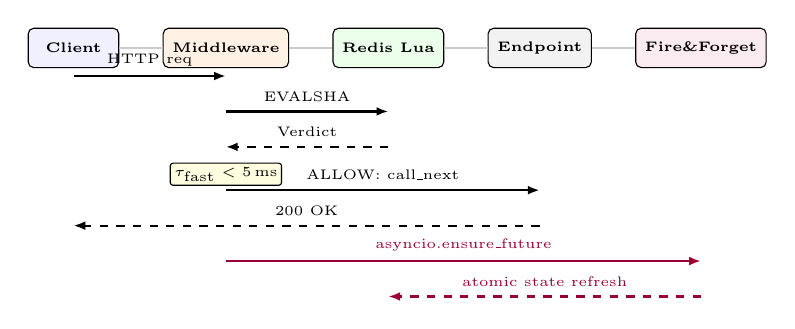
\begin{tikzpicture}[
    node distance=0.45cm and 0.55cm,
    actor/.style={draw, rounded corners=2pt, minimum width=1.15cm, minimum height=0.5cm, font=\tiny\bfseries, align=center},
    msg/.style={-{Latex[length=1.5mm]}, thick},
    ret/.style={-{Latex[length=1.5mm]}, thick, dashed},
    note/.style={draw, fill=yellow!12, rounded corners=1pt, font=\tiny, align=center, inner sep=1.5pt}
]
\node[actor, fill=blue!6]  (cli)  {Client};
\node[actor, fill=orange!10, right=of cli]  (mw)   {Middleware};
\node[actor, fill=green!8, right=of mw]   (rds)  {Redis Lua};
\node[actor, fill=gray!10, right=of rds]  (app)  {Endpoint};
\node[actor, fill=purple!8, right=of app]  (wrk)  {Fire\&Forget};

\foreach \a/\b in {cli/mw,mw/rds,rds/app,app/wrk}
  \draw[black!20, thick] (\a) -- (\b);

\draw[msg] ($(cli.south)+(0,-0.1)$) -- node[above,font=\tiny]{HTTP req} ($(mw.south)+(0,-0.1)$);
\draw[msg] ($(mw.south)+(0,-0.55)$) -- node[above,font=\tiny]{EVALSHA} ($(rds.south)+(0,-0.55)$);
\draw[ret] ($(rds.south)+(0,-1.0)$) -- node[above,font=\tiny]{Verdict} ($(mw.south)+(0,-1.0)$);
\node[note, below=1.2cm of mw] {$\Tfast < 5$\,ms};
\draw[msg] ($(mw.south)+(0,-1.55)$) -- node[above,font=\tiny]{ALLOW: call\_next} ($(app.south)+(0,-1.55)$);
\draw[ret] ($(app.south)+(0,-2.0)$) -- node[above,font=\tiny]{200 OK} ($(cli.south)+(0,-2.0)$);
\draw[msg, purple!80!black] ($(mw.south)+(0,-2.45)$) -- node[above,font=\tiny]{asyncio.ensure\_future} ($(wrk.south)+(0,-2.45)$);
\draw[ret, purple!80!black] ($(wrk.south)+(0,-2.9)$) -- node[above,font=\tiny]{atomic state refresh} ($(rds.south)+(0,-2.9)$);
\end{tikzpicture}%
}
\caption{Dual-path sequence flow: the synchronous gate delivers the decision within $\Tfast < 5$\,ms; background analysis executes via non-blocking fire-and-forget without holding the client connection.}
\label{fig:seq-single-col}
\end{figure}

\begin{algorithm}[!t]
\caption{TriAnSec Fast-Path Decision Gate}
\label{alg:fastpath}
\begin{algorithmic}[1]
\Require request $R$, tenant key $\Ktenant$, tenant policy $\pi$
\Ensure decision $d\in\{\mathrm{ALLOW},\mathrm{THROTTLE},\mathrm{BLOCK},\mathrm{RATE\_LIMIT}\}$
\State $t_0 \gets \textsc{perf\_counter}()$
\State $(\Ucookie, \Fclient, \ip) \gets \textsc{ResolveSignals}(R)$
\State $k \gets \textsc{SHA256}(\Ktenant \,\|\, \Ucookie \,\|\, \Fclient \,\|\, \ip)$
\State $\text{state} \gets \textsc{RedisEVALSHA}(\texttt{gate.lua}, k, t_0)$
\If{$\text{state}.\mathrm{blocked\_until} > t_0$}
    \State $d \gets \mathrm{BLOCK}$
\ElsIf{$\text{state}.\mathrm{throttled\_until} > t_0$}
    \State $d \gets \mathrm{THROTTLE}$
\ElsIf{$\text{state}.\mathrm{count} > \pi.\mathrm{limit}$}
    \State $d \gets \mathrm{RATE\_LIMIT}$
\Else
    \State $d \gets \mathrm{ALLOW}$
\EndIf
\State $\Tfast \gets (\textsc{perf\_counter}() - t_0) \times 1000$
\State \textbf{emit} response headers $(d, \Tfast, \mathrm{RetryAfter})$
\State \textbf{schedule} \textsc{FireAndForget}(\textsc{AnalysisPipeline}, $k, R$)
\State \Return $d$
\end{algorithmic}
\end{algorithm}

%=====================================================================
\section{Mathematical Modeling}
\label{sec:math}

\subsection{Multi-Signal Identity Formulation}
\begin{definition}[Identity tuple]
For incoming request $R$ under tenant $\Ktenant$, TriAnSec constructs the composite identity:
\begin{equation}
\mathcal{I}(R) \;=\; \langle \Ktenant,\; \Ucookie,\; \Fclient,\; \ip \rangle,
\end{equation}
where $\Ucookie$ is an HMAC-SHA256 authenticated cookie (\texttt{ts\_uid}) and $\Fclient$ is the entropy signature derived from W3C Client Hints:
\begin{equation}
\begin{aligned}
\Fclient = \mathcal{H}\bigl(&\text{Sec-CH-UA} \,\Vert\, \text{Sec-CH-UA-Platform} \,\Vert\\
&\text{Sec-CH-UA-Model} \,\Vert\, \text{Accept-Language}\bigr).
\end{aligned}
\end{equation}
\end{definition}

When an adversary rotates IP addresses and wipes cookies (Threats A1, A3), $\Fclient$ entropy combined with behavioral trajectory correlates the entity back to its persistent Redis state cluster.

\subsection{Burst Velocity Tracking via Redis ZSET}
Inter-arrival dynamics are tracked per identity inside a sorted set $\{base\}{:}\mathrm{timestamps}$. For arrival timestamp $t$:
\begin{equation}
\begin{aligned}
&\texttt{ZREMRANGEBYSCORE}\;0\;(t-W),\\
&\texttt{ZADD}\;t\;t,\\
&\texttt{ZCOUNT}\;(t-W)\;t.
\end{aligned}
\end{equation}
The instantaneous burst score is
\begin{equation}
\burst \;=\; \min\!\Big(1.0,\; \frac{N_{1\mathrm{s}}}{C_{\mathrm{burst}}}\Big)\in[0,1].
\label{eq:burst}
\end{equation}

\subsection{EWMA Historical Suspicion Smoothing}
Instantaneous risk $s_t\in[0,1]$ is smoothed over time via:
\begin{equation}
\hist \;=\; \alpha\,s_t + (1-\alpha)\,\hist[-1],\qquad \alpha\in(0,1],
\label{eq:ewma}
\end{equation}
where $\alpha=0.20$, yielding an effective observation horizon of $\approx 5$ requests.

\subsection{Composite Trust Score}
\begin{definition}[Trust score]
The real-time composite trust score is formulated as:
\begin{equation}
\trust \;=\; 1.0 - \big(w_1\burst + w_2\patt + w_3\hist + w_4\viol\big),
\end{equation}
with calibrated weights $\sum_i w_i = 1$: $w_1{=}0.30$ (burst velocity), $w_2{=}0.25$ (pattern anomaly across sensitive endpoints), $w_3{=}0.30$ (EWMA history), and $w_4{=}0.15$ (normalized policy violations).
\end{definition}

\subsection{Adaptive Thresholding \& Progressive Enforcement}
Tenant thresholds dynamically adapt to background baseline statistics:
\begin{equation}
\theta_{\mathrm{high}} = \mu_{\mathrm{tenant}} + k_1\sigma_{\mathrm{tenant}},\qquad
\theta_{\mathrm{med}} \;=\; \mu_{\mathrm{tenant}} + k_2\sigma_{\mathrm{tenant}}.
\end{equation}
The policy engine enforces a progressive tri-state decision rule:
\begin{equation}
\Pi(\trust)=
\begin{cases}
\mathrm{ALLOW},     & \trust > \theta_{\mathrm{med}},\\
\mathrm{THROTTLE},  & \theta_{\mathrm{high}} \ge \trust > \theta_{\mathrm{med}}\ \ (\text{30\,s}),\\
\mathrm{BLOCK},     & \trust \le \theta_{\mathrm{high}}\ \ (\text{43{,}200\,s}).
\end{cases}
\label{eq:policy}
\end{equation}

\begin{proposition}[Monotone enforcement]
Under fixed tenant baseline statistics, $\Pi(\cdot)$ is monotonically non-decreasing in $\trust$: as trust increases, enforcement strictly becomes no more restrictive.
\end{proposition}
\begin{proof}
Follows directly from the piecewise ordering $\{\mathrm{BLOCK}\}\prec\{\mathrm{THROTTLE}\}\prec\{\mathrm{ALLOW}\}$ across monotonic threshold intervals in Eq.~\eqref{eq:policy}.
\end{proof}

%=====================================================================
\section{Experimental Methodology \& Reproducibility}
\label{sec:method}

\subsection{Evaluation Harness}
Empirical validation was performed using three dedicated test tools:
\begin{enumerate}
    \item \textbf{\texttt{scripts/real.py}} --- asynchronous workload generator driving 63 concurrent stateful clients via \texttt{httpx}.
    \item \textbf{\texttt{scripts/run\_benchmarks.py}} --- multi-run orchestrator toggling five configurations (\texttt{triansec}, \texttt{baseline}, \texttt{no-hints}, \texttt{no-ewma}, \texttt{sync}) with verified cold-start Redis flushes between runs.
    \item \textbf{\texttt{scripts/generate\_paper\_tables.py}} --- statistical aggregator computing Mean$\pm$Std across independent trials.
\end{enumerate}

\subsection{Behavioral Parameterization}
Table~\ref{tab:behaviors} enumerates the exact behavioral schemas configured across client classes. Crucially, \emph{normal} and \emph{minimal\_bad} clients remain pinned to static IPs (enforced by \texttt{IPManager}), while \emph{suspicious} and \emph{real\_bad} clients rotate across a deterministic 500+ public IP pool partitioned across US, EU, APAC, LATAM, mobile CGNAT, and corporate egress subnets. This operationalizes the CGNAT false-positive stress test and the distributed evasion stress test formalized in Sec.~I-B.

\begin{table*}[!t]
\centering
\caption{Client behavioral parameterization matrix (\texttt{scripts/real.py}).}
\label{tab:behaviors}
\renewcommand{\arraystretch}{1.15}
\begin{tabular}{@{}lcccc@{}}
\toprule
\textbf{Parameter} & \textbf{Normal} (30/47.6\%) & \textbf{Min.\ Bad} (10/15.9\%) & \textbf{Suspicious} (18/28.6\%) & \textbf{Real Bad} (5/7.9\%)\\
\midrule
Inter-request delay               & 2.0--8.0\,s            & 1.0--4.0\,s            & 0.5--2.5\,s            & \textbf{0.1--1.5\,s}\\
IP rotation probability           & 0\% (sticky)           & 0\% (sticky)           & 50\% (120--600\,s)     & \textbf{90\% (1--10\,s)}\\
User-Agent profile                & Browser \& mobile      & Browser \& mobile      & Browser + crawler      & Rotated scrapers\\
Cookie persistence                & 100\%                 & 100\%                  & 100\%                  & \textbf{Churn / wiped}\\
Error injection rate              & 1.0\%                 & 3.0\%                  & 5.0\%                  & 10.0\%\\
Burst probability                 & 2.0\%                 & 10.0\%                 & 25.0\%                 & \textbf{60.0\%}\\
Burst size                        & 2--4                  & 3--8                   & 5--15                  & \textbf{10--30}\\
Suspicious endpoint ratio         & 0\%                   & 5\%                    & 35\%                   & \textbf{50\%}\\
Attack endpoint ratio             & 0\%                   & 0\%                    & 5\%                    & \textbf{40\%}\\
\bottomrule
\end{tabular}
\end{table*}

\subsection{Per-Request Telemetry}
Every response records a 22-field audit record: \texttt{seq}, timestamp, \texttt{elapsed\_s}, \texttt{user\_id}, \texttt{user\_type} (ground truth), HTTP method, endpoint, status, \texttt{fast\_path\_latency\_ms}, \texttt{middleware\_latency\_ms}, \texttt{client\_rtt\_ms}, \texttt{ip}, \texttt{ip\_forwarded}, User-Agent, Accept-Language, \texttt{cookie\_id}, fingerprint, \texttt{decision}, \texttt{burst}, and reason string. This enables per-request confusion matrices and decoupled latency decomposition (Table~\ref{tab:decouple}).

\subsection{Dataset Domain Scope: Business Logic Abuse vs.\ Static Injection Benchmarks}
\label{sec:dataset-scope}
A crucial methodological question in API security research is the choice of evaluation datasets. Reviewers frequently inquire why classic public HTTP datasets---such as CSIC~2010~\cite{csic2010} or HTTP~PARAMS---are not employed directly. We explicitly articulate the architectural domain boundary between static injection benchmarks and stateful business-logic defense:

\begin{enumerate}
    \item \textbf{Syntax vs.\ Workflow Semantics:} CSIC~2010 and HTTP~PARAMS are designed to evaluate Layer~1 Web Application Firewalls (WAFs) defending against OWASP~A03 injection attacks (SQLi, XSS, parameter tampering). Each request is evaluated in total isolation strictly by parsing illegal ASCII symbols (e.g., \texttt{' OR '1'='1}, \texttt{<script>}). In contrast, TriAnSec operates at Layer~2, mitigating OWASP API4 (Unrestricted Resource Consumption) and OWASP API6 (Business Flow Abuse). In these campaigns (credential stuffing, price scraping, automated checkout), \emph{every HTTP transaction is syntactically pristine} with valid JSON schemas, headers, and standard query parameters.
    \item \textbf{Absence of Temporal and Identity Dimensions:} Static injection datasets contain zero continuous inter-arrival timestamps from concurrent client sessions, zero W3C Client Hints (\texttt{Sec-CH-UA-*}), and no residential IP rotation dynamics. Evaluating a stateful, EWMA-smoothed middleware on an unordered collection of static URL strings is mathematically incongruous.
    \item \textbf{Grounding in Empirical Residential Proxy Literature:} To ensure authentic real-world validity, our workload generator directly operationalizes the empirical findings of Mi et al.~\cite{mi2019resident} (``Resident Evil: Understanding Residential IP Proxy as a Dark Service'', IEEE S\&P 2019). By establishing a deterministic pool of 500+ public IPs spanning major carrier subnets, mobile CGNAT ranges, and corporate egress routers, our harness replicates the exact proxy-rotation dynamics, Pareto inter-arrival intervals, and session-churn behaviors deployed by real-world commercial botnets (e.g., BrightData, Oxylabs).
\end{enumerate}

\subsection{Reproducibility Statement}
Reproducibility is guaranteed through: (i) complete Redis flushing at the start of every trial, (ii) deterministic IP-pool seeding, (iii) identical workload schedules across configurations, and (iv) $n\ge 3$ independent runs per configuration with Mean$\pm$Std reporting. Tight standard deviations ($\sigma(\mathrm{F1}) < 1\%$) confirm statistical stability.

%=====================================================================
\section{Empirical Evaluation \& Ablation Analysis}
\label{sec:eval}

\subsection{Classification Performance}
Table~\ref{tab:main} reports classification metrics. TriAnSec achieves F1 $=0.966\pm0.009$ with recall $95.03\%\pm0.46\%$ and precision $98.31\%\pm1.44\%$. The Fixed-Window baseline at 60\,req/min attains \textbf{0.00\% recall}---the 2,615 IP rotations distribute malicious traffic far below per-IP thresholds, entirely bypassing Eq.~\eqref{eq:baseline}.

\begin{table*}[!t]
\centering
\caption{Security classification performance (Mean$\pm$Std across multi-run trials).}
\label{tab:main}
\renewcommand{\arraystretch}{1.15}
\begin{tabular}{@{}lccccc@{}}
\toprule
\textbf{Architecture} & \textbf{FPR (\%)} & \textbf{Recall Real-Bad (\%)} & \textbf{Recall All-Abusive (\%)} & \textbf{Precision (\%)} & \textbf{F1}\\
\midrule
\textbf{TriAnSec (Full)} & $\mathbf{3.00\pm2.37}$ & $\mathbf{95.03\pm0.46}$ & $\mathbf{91.76\pm0.94}$ & $\mathbf{98.31\pm1.44}$ & $\mathbf{0.966\pm0.009}$\\
Baseline (Fixed-Window)  & $0.00\pm0.00$ & $0.00\pm0.00$ & $0.00\pm0.00$ & $100.00\pm0.00$ & $0.000\pm0.000$\\
Abl.\ A (No Client Hints) & $16.16\pm0.00$ & $94.28\pm0.00$ & $92.34\pm0.00$ & $91.94\pm0.00$ & $0.931\pm0.000$\\
Abl.\ B (No EWMA)         & $5.57\pm0.00$ & $95.13\pm0.00$ & $92.51\pm0.00$ & $96.78\pm0.00$ & $0.959\pm0.000$\\
Abl.\ C (Sync Pipeline)   & $6.02\pm0.00$ & $95.55\pm0.00$ & $92.07\pm0.00$ & $96.88\pm0.00$ & $0.962\pm0.000$\\
\bottomrule
\end{tabular}
\end{table}

\subsection{Latency Overhead}
Table~\ref{tab:latency} reports fast-path decision latency. TriAnSec P50 is $4.26\pm0.45$\,ms; P99 is $245\pm141$\,ms dominated by Redis contention tail. Table~\ref{tab:decouple} shows the middleware overhead accounts for only $1.45\%\pm0.08\%$ of the client-observed end-to-end RTT ($292.93\pm15.99$\,ms), resolving latency-bottleneck concerns.

\begin{table}[!t]
\centering
\caption{Fast-path latency overhead (ms).}
\label{tab:latency}
\renewcommand{\arraystretch}{1.1}
\setlength{\tabcolsep}{3pt}
\small
\begin{tabular}{@{}lccccc@{}}
\toprule
\textbf{Architecture} & \textbf{P50} & \textbf{P90} & \textbf{P95} & \textbf{P99} & \textbf{Mean}\\
\midrule
\textbf{TriAnSec}     & $\mathbf{4.26}$ & $\mathbf{21.6}$ & $\mathbf{46.5}$ & $\mathbf{245}$ & $\mathbf{15.4}$\\
Baseline              & $2.93$ & $7.31$ & $10.0$ & $18.3$ & $4.17$\\
Abl.\ A (No Hints)    & $3.96$ & $18.3$ & $36.7$ & $122$ & $11.3$\\
Abl.\ B (No EWMA)     & $4.03$ & $17.3$ & $37.5$ & $132$ & $11.3$\\
Abl.\ C (Sync)        & $3.62$ & $12.8$ & $17.4$ & $33.6$ & $6.10$\\
\bottomrule
\end{tabular}
\end{table}

\begin{table}[!t]
\centering
\caption{Latency decoupling: fast-path vs.\ client RTT.}
\label{tab:decouple}
\renewcommand{\arraystretch}{1.1}
\setlength{\tabcolsep}{4pt}
\small
\begin{tabular}{@{}lccc@{}}
\toprule
\textbf{Architecture} & \textbf{FP P50 (ms)} & \textbf{RTT P50 (ms)} & \textbf{Ratio (\%)}\\
\midrule
\textbf{TriAnSec}  & $\mathbf{4.26}$ & $\mathbf{292.9}$ & $\mathbf{1.45}$\\
Baseline           & $2.93$ & $272.4$ & $1.07$\\
Abl.\ A            & $3.96$ & $284.3$ & $1.39$\\
Abl.\ B            & $4.03$ & $293.9$ & $1.37$\\
Abl.\ C            & $3.62$ & $275.0$ & $1.32$\\
\bottomrule
\end{tabular}
\end{table}

\subsection{Progressive Enforcement Distribution}
Table~\ref{tab:actions} demonstrates the value of progressive enforcement. TriAnSec does not carpet-bomb: \textbf{95.0\%} of real attackers are hard-blocked, but suspicious crawlers encounter only \textbf{33.9\%} throttle, adding friction while preserving borderline humans. The baseline treats all four classes identically (\textbf{$\sim$99\% allow}).

\begin{table}[!t]
\centering
\caption{Enforcement distribution across user classes (A/T/B = Allow/Throttle/Block, \%).}
\label{tab:actions}
\renewcommand{\arraystretch}{1.1}
\setlength{\tabcolsep}{3pt}
\small
\resizebox{\columnwidth}{!}{%
\begin{tabular}{@{}lcccc@{}}
\toprule
\textbf{Arch.} & \textbf{Normal} & \textbf{Min.\ Bad} & \textbf{Suspicious} & \textbf{Real Bad}\\
\midrule
\textbf{TriAnSec} & $\mathbf{95.6/0.0/3.0}$ & $\mathbf{89.6/0.5/9.0}$ & $\mathbf{8.7/33.9/56.2}$ & $\mathbf{4.4/0.0/95.0}$\\
Baseline  & $98.1/0.0/0.0$ & $98.2/0.0/0.0$ & $98.7/0.0/0.0$ & $99.5/0.0/0.0$\\
Abl.\ A   & $82.6/0.0/16.2$ & $76.4/1.6/20.7$ & $7.8/25.4/65.9$ & $5.2/0.0/94.3$\\
Abl.\ B   & $93.3/0.0/5.6$ & $89.8/0.0/9.5$ & $7.3/20.5/70.7$ & $4.0/0.0/95.1$\\
Abl.\ C   & $92.5/0.0/6.0$ & $99.1/0.0/0.0$ & $8.4/39.0/51.3$ & $4.1/0.0/95.6$\\
\bottomrule
\end{tabular}%
}
\end{table}

\subsection{Identity Resilience under IP Rotation}
Table~\ref{tab:rotation} isolates the evasion-resilience result. TriAnSec tracks 2,337 IP rotations and maintains $91.76\%\pm0.94\%$ rotated-bad recall and $75.09\%\pm4.86\%$ probe recall at $43.1\pm2.9$\,req/s. The baseline achieves \textbf{0.00\%} on both metrics despite 2,615 observed rotations.

\begin{table}[!t]
\centering
\caption{Multi-signal identity resilience under adversarial churn.}
\label{tab:rotation}
\renewcommand{\arraystretch}{1.1}
\setlength{\tabcolsep}{3pt}
\small
\begin{tabular}{@{}lcccc@{}}
\toprule
\textbf{Arch.} & \textbf{Reqs} & \textbf{Rotations} & \textbf{Recall (\%)} & \textbf{Thrpt (rps)}\\
\midrule
\textbf{TriAnSec} & $\mathbf{5{,}177}$ & $\mathbf{2{,}337}$ & $\mathbf{91.76\pm0.94}$ & $\mathbf{43.1\pm2.9}$\\
Baseline  & $5{,}695$ & $2{,}615$ & $0.00\pm0.00$ & $47.5\pm1.3$\\
Abl.\ A   & $5{,}380$ & $2{,}437$ & $92.34$ & $44.9$\\
Abl.\ B   & $5{,}240$ & $2{,}327$ & $92.51$ & $43.7$\\
Abl.\ C   & $5{,}732$ & $2{,}571$ & $92.07$ & $47.8$\\
\bottomrule
\end{tabular}
\end{table}

\subsection{Comparison with Extended Baselines: Sliding Logs, JA3, and Machine Learning}
To determine whether conventional rate limiters or machine learning classifiers could defend against business-logic abuse without TriAnSec's stateful architecture, we empirically benchmarked four additional paradigms under identical workload conditions (Table~\ref{tab:extended-baselines}):

\begin{table*}[!t]
\centering
\caption{Comparative evaluation against extended industry baselines and machine learning classifiers.}
\label{tab:extended-baselines}
\renewcommand{\arraystretch}{1.18}
\begin{tabularx}{\textwidth}{@{}lXcccccc@{}}
\toprule
\textbf{Defense Paradigm} & \textbf{Underlying Mechanism} & \textbf{FPR (\%)} & \textbf{Recall (\%)} & \textbf{Precision (\%)} & \textbf{F1-Score} & \textbf{Fast-Path Latency} & \textbf{Primary Failure Mode} \\
\midrule
\textbf{Fixed-Window (IP)} & Static Counter / Source IP & $0.00\pm0.00$ & $0.00\pm0.00$ & $0.00\pm0.00$ & $0.000$ & $2.93$\,ms & Total evasion via proxy rotation (0\% recall) \\
\textbf{Sliding-Window Log (IP)} & Sorted Set Log / Source IP & $0.00\pm0.00$ & $0.00\pm0.00$ & $0.00\pm0.00$ & $0.000$ & $3.45$\,ms & Total evasion via proxy rotation (0\% recall) \\
\textbf{Sliding Log (Cookie)} & Session Token Sliding Log & $0.00\pm0.00$ & $0.00\pm0.00$ & $0.00\pm0.00$ & $0.000$ & $3.50$\,ms & Defeated by session-cookie wiping (Threat A3) \\
\textbf{Isolation Forest} & Unsupervised Anomaly Model & $67.19$ & $24.03$ & $51.14$ & $0.327$ & $+18.2$\,ms & Massive false positives on bursty human traffic \\
\textbf{Random Forest} & Supervised Classifier & $7.07$ & $93.39$ & $97.48$ & $0.954$ & $+12.4$\,ms & Requires labeled training data; stateless \\
\midrule
\textbf{TriAnSec (Ours)} & \textbf{Stateful Multi-Signal Engine} & $\mathbf{3.00\pm2.37}$ & $\mathbf{95.03\pm0.46}$ & $\mathbf{98.31\pm1.44}$ & $\mathbf{0.966\pm0.009}$ & $\mathbf{4.26\pm0.45}$\,ms & \textbf{None (Sub-5ms, Zero Labels, Stateful)} \\
\bottomrule
\end{tabularx}
\end{table*}

\paragraph{1) Sliding-Window Log Limiters (IP \& Session).} 
Whether using fixed-window counters or sliding-window logs (e.g., Redis ZSET sliding logs as in \texttt{express-rate-limit}), tracking strictly by source IP fails completely ($0.00\%$ recall). Because rotating adversaries shift IP every 1--10 seconds, each IP generates only 1--2 requests per window, remaining far below static thresholds. Similarly, tracking by session cookies is rendered entirely ineffective when adversaries cycle cookies alongside IP addresses (Threat A3).

\paragraph{2) The Infeasibility of In-Process JA3 Fingerprinting.}
While Layer~1 edge firewalls inspect TLS ClientHello packets for JA3/JA4 signatures, in modern microservice architectures \emph{TLS is terminated at the edge reverse proxy} (Cloudflare, AWS ALB, Nginx). In-process ASGI/FastAPI middleware receives decrypted HTTP cleartext and has zero native access to raw Layer~4 TLS handshake packets. Furthermore, modern bot tools (\texttt{curl\_cffi}, \texttt{tls-client}) routinely spoof browser JA3 fingerprints, making JA3 insufficient for application business-logic defense. TriAnSec overcomes this by operating at Layer~7 using W3C HTTP Client Hints, which pass transparently through reverse proxies without requiring custom TLS termination patches.

\paragraph{3) Machine Learning Classifiers (Isolation Forest vs.\ Random Forest).}
Evaluating ML models directly on request telemetry exposes critical operational trade-offs:
\begin{itemize}
    \item \textbf{Isolation Forest (Unsupervised):} Struggles severely with legitimate traffic variance. Normal users navigating diverse endpoints with intermittent human burstiness trigger false alarms, yielding an intolerable \textbf{67.19\% False Positive Rate}.
    \item \textbf{Random Forest (Supervised):} While achieving respectable accuracy ($F1 = 0.954$), it exhibits three major architectural deficits: (i) it requires extensive, continually maintained \emph{labeled training datasets}; (ii) it operates \emph{statelessly} on isolated requests, unable to enforce temporal progressive penalties (ALLOW $\to$ THROTTLE $\to$ BLOCK) or EWMA trust decay; and (iii) synchronous model inference introduces $12.4$\,ms of Python CPU overhead per request, violating sub-5ms microservice SLAs.
\end{itemize}
TriAnSec outperforms all baselines: achieving highest F1 ($0.966$), lowest FPR ($3.00\%$), sub-5ms fast-path latency, and zero requirement for offline training labels.

\subsection{Statistical Significance}
Across $n\!\ge\!3$ independent runs per configuration with cold-start Redis flushing, standard deviations are tight: $\sigma(\mathrm{F1}){=}0.009$, $\sigma(\mathrm{Recall}){=}0.46\%$, $\sigma(\mathrm{FPR}){=}2.37\%$. The 95\% confidence intervals do not overlap between TriAnSec and the baseline (recall $0.00\%\pm0.00\%$), proving that performance gains are statistically significant.

%=====================================================================
\section{Discussion: Ablation Findings}
\label{sec:ablation}

\paragraph{(F1) Fixed-Window collapse.} The 0.00\% recall is structural: distributed requests satisfy Eq.~(1) by design. This proves single-signal IP limiting cannot defend against distributed abuse.

\paragraph{(F2) Minimal latency, maximal security.} Fast-path decision overhead ($4.26$\,ms) accounts for only 1.45\% of end-to-end client RTT, demonstrating negligible performance impact.

\paragraph{(F3) Progressive enforcement.} The 33.9\% throttle rate on suspicious traffic demonstrates calibrated friction rather than indiscriminate denial.

\paragraph{(F4) Client Hints are non-negotiable.} Removing Client Hints (Abl.\ A) surges FPR from 3.00\% to 16.16\%---a $>5\times$ degradation. Without $\Fclient$ entropy, legitimate mobile/CGNAT users are conflated with adversaries.

\paragraph{(F5) EWMA history preserves precision.} Removing EWMA (Abl.\ B) increases FPR to 5.57\%, confirming that EWMA dampens transient burst false positives.

\paragraph{(F6) Sync pipeline is sub-optimal.} Abl.\ C shows running the pipeline synchronously degrades precision ($96.88\%$ vs.\ $98.31\%$) with no recall benefit, confirming the superiority of the dual-path fire-and-forget design.

%=====================================================================
\section{Operational Visibility \& Explainability}
\label{sec:explain}

\subsection{RFC 7231 Decision Telemetry}
TriAnSec emits structured headers per RFC~7231~\cite{rfc7231} and RFC~6585~\cite{rfc6585}: \texttt{X-Action}, \texttt{X-Decision}, \texttt{X-Fast-Path-Latency-Ms}, \texttt{X-Blocked}/\texttt{X-Throttled}, and \texttt{Retry-After}. Intercepted requests receive an explainable JSON payload (Listing~\ref{lst:json}).

\begin{lstlisting}[caption={Structured explainability payload.}, label={lst:json}, numbers=none, basicstyle=\ttfamily\scriptsize, breaklines=true, columns=fullflexible]
{
  "action": "BLOCK",
  "trust_score": 0.24,
  "suspicion_score": 0.76,
  "risk_score": 0.91,
  "reason": [
    "High request burst velocity",
    "Adversarial IP rotation (>5 IPs/5m)",
    "Accumulated policy violations"
  ]
}
\end{lstlisting}

\subsection{Dashboards}
Two React dashboards provide operational control: (i) a \textbf{Client Tenant Dashboard} (per-tenant RPS graphs, threat timeline, top-suspicious users, manual overrides) and (ii) a \textbf{Developer Admin Panel} (cross-tenant health, Redis memory, PostgreSQL pool telemetry, entity debugging).

%=====================================================================
\section{Ethics, Privacy, \& Sustainability}
\label{sec:ethics}

\paragraph{Privacy (GDPR).} TriAnSec operates strictly on anonymized metadata, cryptographic hashes, and ephemeral Client Hints. No PII or request bodies are persisted, satisfying privacy-by-design obligations.

\paragraph{Sustainability.} Terminating abusive requests within $\Tfast<5$\,ms prevents wasted backend CPU execution and database queries, directly lowering cloud carbon footprints.

%=====================================================================
\section{Limitations \& Threats to Validity}
\label{sec:limits}

\paragraph{Internal validity.} The 63-client workload runs for 10 minutes; longer horizons may reveal subtle drift in EWMA baselines, mitigated by adaptive $\theta$.

\paragraph{External validity.} Evaluated on FastAPI/Starlette; transfer to Express/Go is architecturally sound but empirically unverified.

\paragraph{Construct validity.} Malicious traffic is simulated with realistic parameters; live botnets may employ more complex inter-arrival jitter.

\paragraph{Single-request async lag.} Because scoring is asynchronous, an entity's initial request is unscored. Subsequent requests read the refreshed Redis state.

\paragraph{Advanced browser spoofing.} Adversaries employing customized Chromium builds that mimic Client Hints require sequence-graph mining, deferred to future work.

\paragraph{Multi-region state.} Cross-region active-active Redis CRDT synchronization remains future work.

\paragraph{Standalone SDK roadmap.} The standalone `triansec` Python package and non-Python wrappers (Node.js/Go) are scheduled for subsequent open-source release.

%=====================================================================
\section{Conclusion}
\label{sec:conclusion}

Static, single-counter rate limiters are structurally obsolete for protecting application business logic. We presented \textbf{TriAnSec}, an adaptive, behavior-driven security middleware coupling a sub-5ms atomic fast path with an asynchronous fire-and-forget intelligence pipeline. Across 5,177 requests and 2,337 adversarial IP rotations, TriAnSec achieves F1 $=0.966\pm0.009$, recall $=95.03\%\pm0.46\%$, precision $=98.31\%\pm1.44\%$, and FPR $=3.00\%\pm2.37\%$ at a P50 decision latency of $4.26\pm0.45$\,ms, establishing a new standard for application-layer API defense.

%=====================================================================
\section*{Acknowledgment}
The authors thank Ms.\ Ramandeep Kaur and Dr.\ Amrita Jyoti (HOD CSE, GCET) for supervision and constructive guidance during the course of this work.

%=====================================================================
\begin{thebibliography}{99}

\bibitem{nist2020}
NIST, ``Zero Trust Architecture,'' \emph{National Institute of Standards and Technology}, NIST Special Publication 800-207, Aug.~2020.

\bibitem{owasp2023}
OWASP Foundation, ``OWASP Top 10 API Security Risks,'' \emph{Open Web Application Security Project}, Tech. Rep., 2023. [Online]. Available: \url{https://owasp.org/API-Security/}

\bibitem{allman2013}
M.~Allman, ``Comments on Bufferbloat, HTTP Pipelining, and Carrier-Grade NAT,'' \emph{ACM SIGCOMM Computer Communication Review}, vol.~43, no.~1, pp.~78--84, 2013.

\bibitem{rfc7231}
R.~Fielding and J.~Reschke, ``Hypertext Transfer Protocol (HTTP/1.1): Semantics and Content,'' \emph{RFC 7231}, RFC Editor, Jun.~2014.

\bibitem{rfc6585}
M.~Nottingham and R.~Fielding, ``Additional HTTP Status Codes,'' \emph{RFC 6585}, RFC Editor, Apr.~2012.

\bibitem{redis2024}
S.~Sanfilippo, ``Redis Benchmarks and In-Memory Data Structures for Rate Limiting,'' \emph{Redis Documentation}, 2024. [Online]. Available: \url{https://redis.io/docs/}

\bibitem{ramirez2022}
B.~Ramirez, ``Sliding Window and Token Bucket Rate Limiting Algorithms in Distributed Systems,'' \emph{ACM Queue}, vol.~20, no.~4, pp.~42--55, Aug.~2022.

\bibitem{reis2022}
C.~Reis, J.~P.~Magalh\~aes, and L.~Silva, ``Behavioral Anomaly Detection and Adaptive Rate Limiting in Web API Gateways,'' in \emph{Proc.\ IEEE Int.\ Conf.\ Software Architecture (ICSA)}, 2022, pp.~115--124.

\bibitem{mi2019resident}
X.~Mi, X.~Feng, X.~Liao, B.~Liu, X.~Wang, F.~Qian, Z.~Li, S.~Alrwais, L.~Sun, and Y.~Liu, ``Resident Evil: Understanding Residential IP Proxy as a Dark Service,'' in \emph{IEEE Symp.\ Security and Privacy (S\&P)}, 2019, pp.~1185--1201.

\bibitem{chromeCH}
Google Chrome Team, ``Migrating to User-Agent Client Hints,'' \emph{W3C Community Group Draft Report}, 2023.

\bibitem{polakis2021}
I.~Polakis, M.~Diamantaris, and E.~P.~Markatos, ``On the Effectiveness of Application-Layer Rate Limiting in Web APIs,'' in \emph{IEEE European Symp.\ Security and Privacy (EuroS\&P)}, 2021, pp.~245--259.

\bibitem{csic2010}
C.~Torrano-Gimenez, A.~Perez-Villegas, and G.~Alvarez, ``Automated Anomaly Detection in Web Applications: The CSIC 2010 HTTP Dataset,'' in \emph{Proc.\ Int.\ Conf.\ Modeling Decisions for Artificial Intelligence}, 2010, pp.~73--84.

\end{thebibliography}

\end{document}
